\section{BSM Physics Interpretation}
\label{sec:bsm}

\subsection{BSM Models}
\label{sec:bsmmodels}

As is clear from Table~\ref{resulttable}, we see no excess yield above the background prediction.
We thus interpret the results in the context of models characterized by the 
production of charginos and neutralinos.
We calculate upper limits on the cross sections times branching fractions into the \wzmet\ and \zzmet\
final states as a function of the chargino and neutralino masses. 
We interpret our limits in the context of two %three 
SUSY models:

\begin{itemize}
\item WZ SMS: $\chi^{\pm}_{1}\chi^{0}_{2} \rightarrow$\wzmet
%\item ZZ SMS: $\chi^{0}_{2}\chi^{0}_{3} \rightarrow$\zzmet
\item A GMSB model with large branching fraction to \zzmet~\cite{ref:ewkino}
\end{itemize}

For the WZ %and ZZ 
SMS model, %s, 
it is assumed that $m_{\chi^{\pm}_1} = m_{\chi_2^0} = m_{\chi_3^0} \equiv m_\chi$,
and that the chargino (neutralino) decays to $W+\rm{LSP}$ ($Z+\rm{LSP}$) with a branching fraction of 100\%,
where the LSP is the lightest neutralino $\chi^{0}_{1}$. 
%Because the  $\chi^{0}_{2}\chi^{0}_{3}$ production
%cross section is very small, our analysis does not have sensitivity to the ZZ SMS model.
We also interpret our results in the context of a general gauge-mediated symmetry breaking (GGMSB) 
Z-enriched higgsino model~\cite{ref:ewkino}, which has a large branching fraction to the \zzmet\ final 
state. In this scenario, the LSP is the gravitino which is very light (mass $\leq$ 1 keV).
Systematic uncertainties in the background estimate (Sec.~\ref{sec:systematics}) and signal efficiency
and acceptance (Sec.~\ref{sec:acc_systematics}), are incorporated into the limits.
See Appendix \ref{sec:app_bsm} for interpretation results in the ZZ SMS model.

\input{accept_systematics.tex} %move to SMS as subsection

\clearpage

\subsection{Exclusion Procedure}

Our interpretation for the models discussed in Sec.~\ref{sec:bsmmodels} is based on a ``shape analysis,'' using the results in multiple, exclusive
\MET\ regions as summarized in Table~\ref{resulttableex}. 
The exclusion is performed using the LHC-type CLs method as implemented in LandS.
The systematic uncertainties on the background (see Sec.~\ref{sec:systematics}) are assessed separately for each of the
three background contributions (\zjets\ bkg, OF bkg, WZ/ZZ bkg), and are assumed to be 100\% correlated across all five
exclusive signal regions. For the signal efficiency uncertainties, the lepton selection (2\%/lepton), trigger efficiency (2\%),
integrated luminosity (2.2\%), and b-tagging efficiency (4\%) are assessed for each model point. 

The uncertainties related to jets and \MET\ quantities (jet multiplicity, dijet mass, and \MET) vary significantly across 
the BSM model parameter space, and are addressed separately at each point using the procedure of Sec.~\ref{sec:acc_systematics}.
These uncertainties are implemented using the ``shape morphing'' technique which takes into account the bin-to-bin migration
of signal events.

\subsection{Results of BSM Interpretation}
\label{sec:bsmresults}

In Fig.~\ref{fig:limits}, we compare the observed cross section upper limits with the theory predictions
for the WZ SMS (left) %, ZZ SMS, 
and GMSB model (right).
For the WZ %and ZZ SMS models, 
model, the cross section upper limit is calculated for the cases of LSP masses 0 GeV and 50 GeV.
For the WZ SMS model, the signal cross section is indicated separately for pure wino-like and higgsino-like couplings. 
The wino-like scenario corresponds to purely diagonal neutralino and chargino mixing matrices, leading to an effective coupling
of $g\gamma^{\mu}$ at the $W^*\chi^{\pm}\chi^{0}$ production vertex, where $g$ is the electroweak coupling.
In the higgsino-like scenario the two lightest neutralinos consist of equal admixtures of the two neutral higgsinos which are
assumed to have equal mass; in this scenario the couping is reduced to $g\gamma^{\mu}/\sqrt{2}$.
All signal cross sections are calculated with {\sc prospino} 2.1, and are summarized in Tables~\ref{chiwzsigeff} (WZ SMS)
%, \ref{chizzsigeff} (ZZ SMS),
and \ref{hsigeff} (GMSB model).

For the WZ SMS model in the wino-like scenario with massless LSP, our results exclude the range $m_{\chi}$ 
149--207~GeV\footnote{The $m_\chi$ exclusion range will degrade slightly after taking into account the uncertainty on the cross section
from PDF and renormalization/factorization scale, which will be added shortly. Since the relevant mass scale is low, and this is an electroweak production
process, this uncertainty is expected to be small.}, under the assumptions that
$\rm{BR}(\chi^{\pm}\chi^{0}\to \rm{WZ}+\MET)=1$.
We do not exclude any region of $m_{\chi}$ for the case of 50 GeV LSP mass.
Due to the reduced coupling in the higgsino-like scenario, our results do not exclude any range of $m_\chi$.

For the ZZ SMS model, we do not exclude any region of $m_{\chi}$ (see App. \ref{sec:app_bsm}).
This is due to the fact that in the MSSM, neutralino pair production is suppressed relative to neutralino-chargino production.
Therefore, our results are not sensitive to a scenario in which neutralino pair production is the sole production mechanism.
However, the \zzmet\ signature may be enhanced in scenarios in which additional production mechanisms, eg. chargino-chargino and chargino-neutralino,
also contribute. This is the case in a GMSB Z-enriched higgsino model~\cite{ref:ewkino}. In this scenario, the LSP is a nearly massless
gravitino, the next-to-lightest SUSY particle (NLSP) is a Z-enriched higgsino $\chi^0_1$ and the $\chi^{\pm}$ is nearly mass degenerate with the $\chi^{0}_{1}$. 
Hence the $\chi^{\pm}$ decays to a $\chi^{0}_{1}$ and to low \pt SM particles which escape detection. Thus, all production mechanisms
(chargino-chargino, chargino-neutralino, and neutralino-neutralino) lead to a pair of $\chi^{0}_{1}$ particles in the final state, and the branching fraction
to \zzmet\ is large (varying from 100\% at $m_\chi=130$~GeV to 85\% at $m_\chi=410$~GeV, as summarized in Table~\ref{hsigeff}).
As indicated in Fig.~\ref{fig:limits}, our results exclude the range  $m_{\chi}$ 155--233~GeV
in this scenario\footnote{The same caveat applies here.}.

\begin{figure}[th!]
  \begin{center}
    \includegraphics[width=0.49\textwidth]{plots/WZnew.pdf}
    %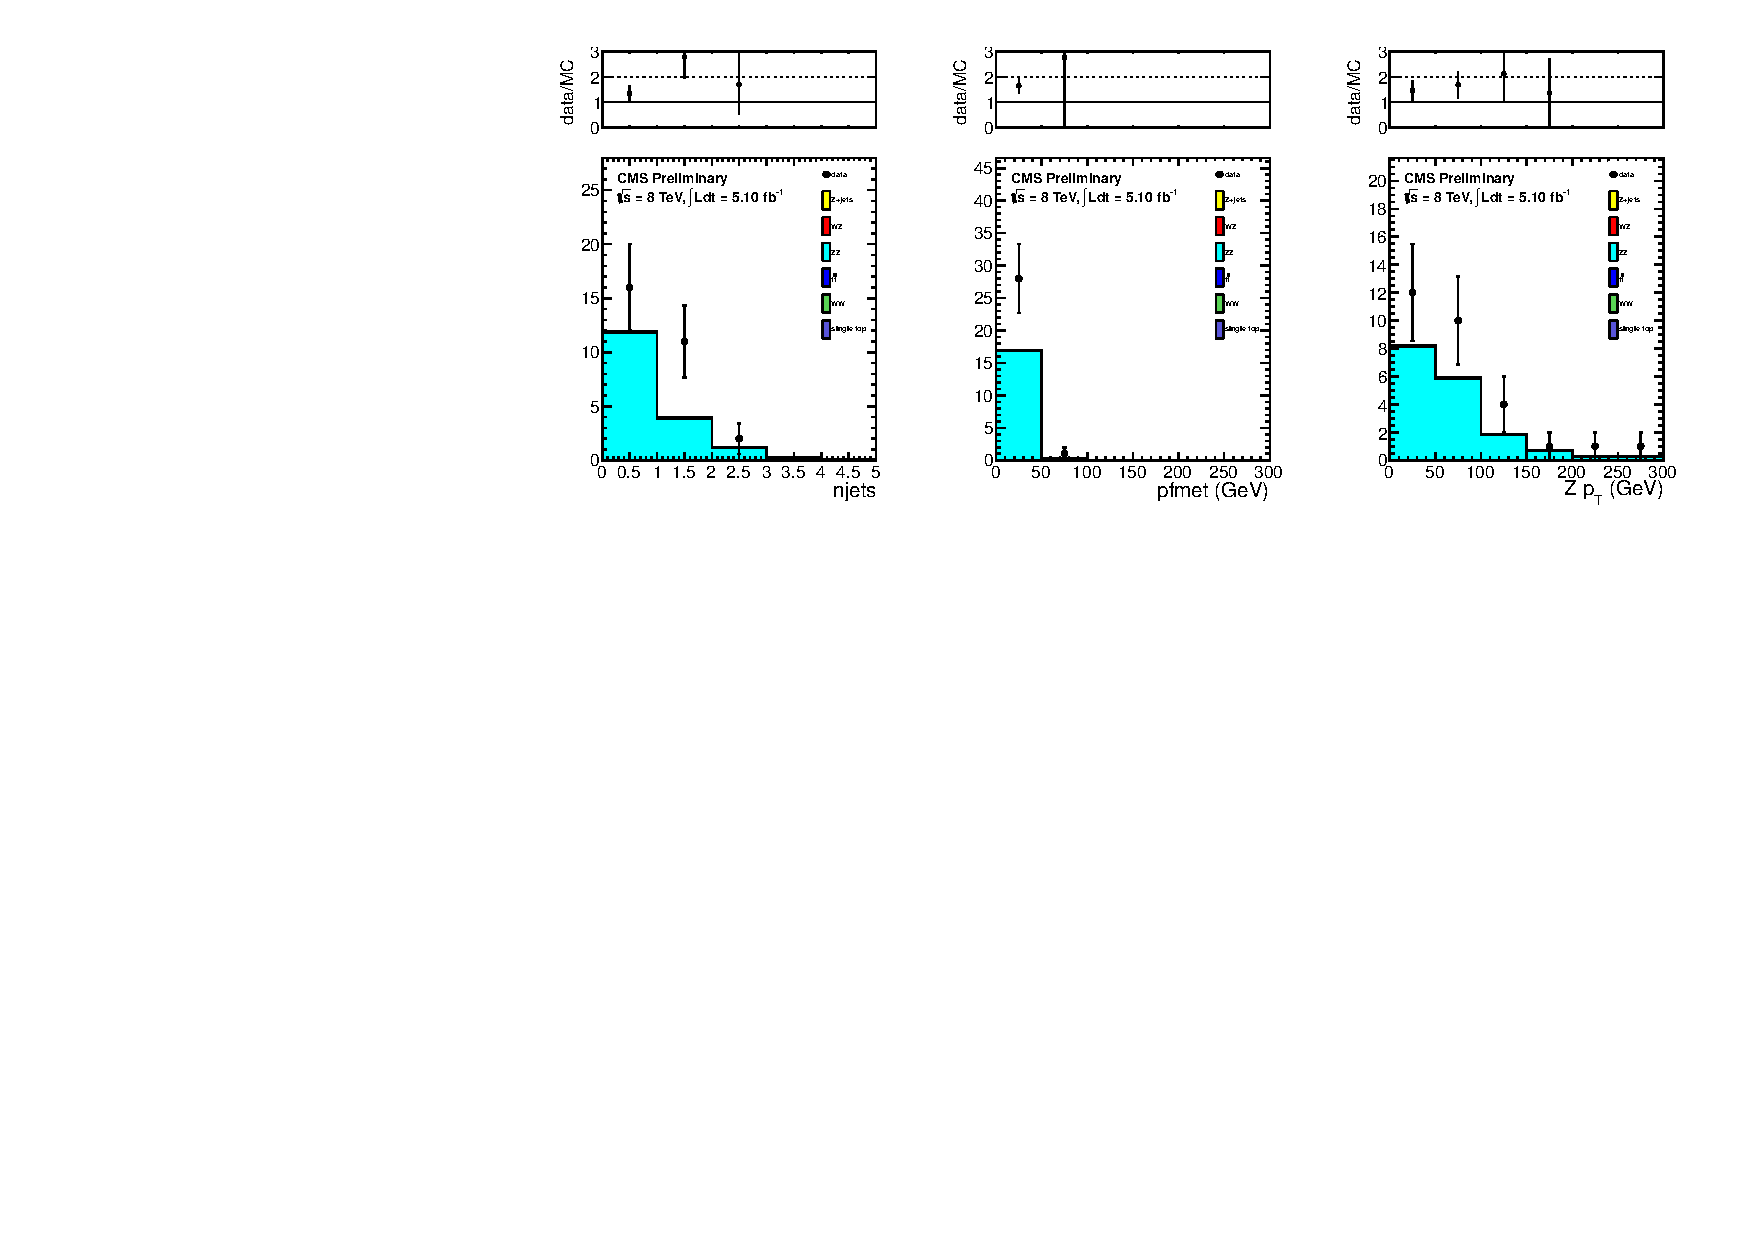
\includegraphics[width=0.49\textwidth]{plots/ZZ.pdf}
    \includegraphics[width=0.49\textwidth]{plots/GMSB.pdf}
    \caption{
      Interpretation in the WZ SMS (left) %(upper left), ZZ SMS (upper right), 
	  and GMSB model (right). % (bottom).
      The observed cross section upper limits (red contours) are compared with the theory predictions (blue contours).
      For the WZ %and ZZ 
	  SMS model, %s, 
	  we display the observed cross section limits for massless LSP (solid red contour) and LSP with mass 50 GeV (dotted contour).
	  We also
      %For the WZ model we 
	  display both the wino-like (solid blue contour) and higgsino-like (dashed blue contour) (see text for details).
      For the GMSB model the excluded region $m_{\chi}$ 155--233~GeV is indicated by the gray shaded box.
      \label{fig:limits}
    }
  \end{center}
\end{figure}

In Fig.~\ref{fig:2Dlimits} we display the signal efficiency times acceptance and the observed cross section upper limits
in the 2-dimensional SMS parameter space.

\begin{figure}[th!]
  \begin{center}
    \includegraphics[width=0.9\textwidth]{plots/WZ_2D.pdf}
    %\includegraphics[width=0.9\textwidth]{plots/ZZ_2D.pdf}
    \caption{
      Interpretation in the WZ SMS model. % (top) and ZZ SMS model (bottom).
      The signal efficiency times acceptance to pass the \MET\ $>$ 60 GeV signal region requirement is indicated in the left plot. %s.
      The observed 95\% CL cross section upper limits are indicated in the right plot. %s. 
	  %For the WZ SMS model, 
	  The solid contour in this plot
      indicates the excluded region, assuming the pure wino-like cross section.
      \label{fig:2Dlimits}
    }
  \end{center}
\end{figure}

Additional interpretation results are presented in the appendices.
In App.~\ref{app:combo}, we combine the results of this search with those of the Rutgers/KIT
multi-lepton analysis SUS-11-013 and interpret the results in the GMSB model.
In App.~\ref{app:combo_trilepton}, we combine the results of this search with those of the Florida/UCLA
trilepton analysis and interpret the results in the WZ SMS model.

%restore when updated

%\begin{figure}[th!]
%  \begin{center}
%    \includegraphics[width=1.0\textwidth]{plots/zz4.pdf}
%    \caption{
%	  95\% CLs cross section upper limit (red) and 
%	  model cross sections (blue) as a function of mass parameter. See text for more details.
%	  \label{fig:zzLimits}
%	}
%  \end{center}
%\end{figure}

%\begin{table}[htb]
%  \begin{center}
%	\caption{\label{tab:xsections} 
%	Reference cross sections for the \wzmet\ and \zzmet\ models as a function of the mass parameter $m_{\chi}$.
%	}
%\begin{tabular}{l|cc|c}
%\hline
%\hline
% & \multicolumn{2}{c|}{\wzmet} & {\zzmet} \\
%$m_{\chi}$ (GeV) & $\sigma_{wino}$ (fb) & $\sigma_{higgsino}$ (fb) & $\sigma$ (fb) \\
%\hline
%200 & 611 & 313 & 82 \\
%220 & 410 & 211 & 55 \\
%240 & 283 & 145 & 37 \\
%260 & 199 & 104 & 26 \\
%280 & 144 & 74  & 19 \\
%300 & 104 & 55  & 14 \\
%\hline
%\hline
%
%\end{tabular}
%\end{center}
%\end{table}


%%%%%%%%%%%%%%%%%%%%%%%%%%%%%%%%%%%%%%%%%%%%%%%%%%%%%%%%%%%%%%%%%%55
